%\documentclass[a4paper,10pt]{report}
\documentclass[11pt,titelpage]{scrreprt}
\usepackage[utf8]{inputenc}
\usepackage[ngerman]{babel}
\usepackage{graphicx}
\usepackage{fancyhdr}
\usepackage{fancyref}
\usepackage{lscape}

  
%must be before gloassary stuff\usepackage{hyperref} 
\usepackage[toc]{glossaries} 
\glsaddall
\makeglossaries

\newglossaryentry{computer}
{
  name=computerLST,
  description={is a programmable machine that receives input,
               stores and manipulates data, and provides
               output in a useful format}
} 

  

% Title Page
\title{Alarm Clock }
\author{Jonathan Hyams \\Pascal Schmalz}
\titlehead{\centering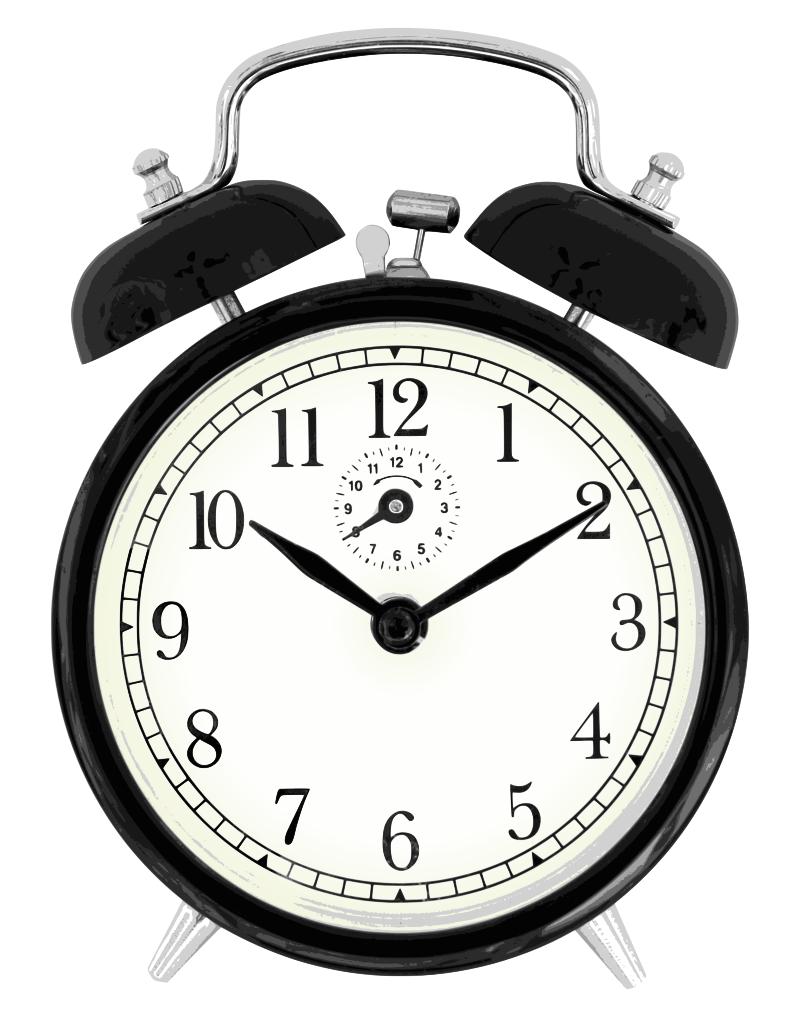
\includegraphics[width=6cm]{img/clock.png}}

%Make the Header
\makeatletter
\let\runauthor\@author
\let\runtitle\@title
\makeatother
\rhead{\runauthor}
\chead{\runtitle}
\lhead{\begin{picture}(0,0) \put(0,0){
\includegraphics[scale=0.5]{img/bfh.png}} \end{picture}}



\begin{document}

\thispagestyle{empty}
\maketitle
\tableofcontents

\pagestyle{fancy}


\begin{abstract}
\end{abstract}
\section{Zweck des Dokument}
TODO this is new text
\gls{computer}
%makes sure the whole glossary gets printed even when acronyms are not defined

\section{Kurzbeschreibung}
Das Ziel des Projektes ist einen Ersatz zum Programm kAlarm zu entwickeln.
Das Program kAlarm erlaubt es den User Benutzerdefinierte Erinnerungen zu erstellen. Mittels Pop-Up Windows wird der User dann zur gegebenen Zeit daran erinnert.
Im gegensatz zu kAlarm soll das zu erstellende Produkt Platformübergreifend verfügbar sein. Wie kAlarm soll dieses Produkt unter einer Open Source Lizenz entwickelt werden.
\section{Projektziele}
Unser Auftraggeber ist kein Unternehmen. Es werden somit auch keine Ziele innerhalb einer Unternehmens verfolgt.
Ziele welche ein Benuzer unsere Aplikaiton verfolgen könnte wären Beispielsweise:
\begin{itemize}
 \item Wiederkehrende Events nicht zu vergessen.
 \item An den Wäscheta erinnert weden.
 \item Die Wäsche rechtzeitig aus de Wäscheküche holen.
\item Den Kuchen nicht im Backofen verbrennen lassen.
 \item Der Sekretärin zum Geburtstag Blumen schicken.
 
\end{itemize}

\section{Stakeholders}
\begin{itemize}
\item{Auftragsgeber: Prof. Claude Furrer}
\item{Auftragsnehmer: Jonathan Hyams, Pascal Schmalz}
\item{Benutzer: FOSS Communitiy}
\end{itemize}
\section {Systemabgrenzung}
\subsection{Geschäftsprozesse}
Es existieren keine vor\- oder nachgelagerten Prozesse. Unsere Lösung lässt sich in beliebige viele Prozesse integrieren.
\subsection{Systeme}
Unser System wirkt mit Datebanken zusammen. Es baut auf Betriebsystemskomponenten auf. Namentlich Cronjob /Schtasks.
%TODO uml einbinden
\begin{landscape}
\begin{figure}
  \centering
    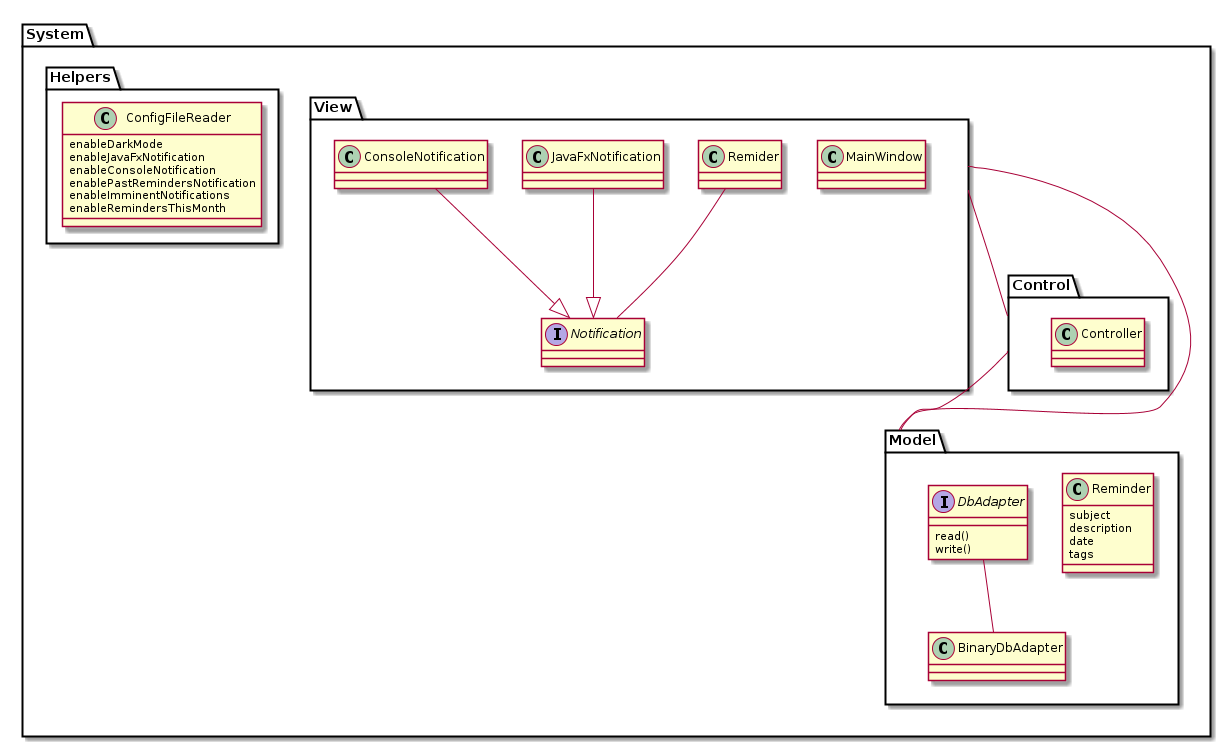
\includegraphics[width=1\textwidth]{../uml/uebersicht.png}
  \caption{Systemübersicht und Abgrenzung}
  \label{fig:overview}
\end{figure}
\end{landscape}
Die Systemübersicht und Abgrenzung Abb.~\ref{fig:overview} Seite~\pageref{fig:overview} bedient sich der UML Notation, ohne die UML Spezifikationvollständig einzuhalten.
\pageref{fig:overview}
 





Je nach gewünschter Notification Möglichkeiten kann mit E-Mails, SMS und Systemnotifications gearbeitet werden.Dies Bedingut, dass entsprechende Services / Server eingerichtet und über eine definierte Schnittschtelle erreichbar sind.
\subsection{Randbedingungen}
Die Entwicklung soll mittls Java und JavaFX erfolgen.
Das Prgoramm soll Betriebssystem und Datenbank agnostisch sein. Das Projekt muss unter einer Opensource Lizenz veröffentlicht werden.
Die Dokumentation muss in \LaTeX erstellt werden.


\subsection{Prozessumfeld}
\subsection{Systemumfeld}
\subsection{Randbedingungen}
\section{Anforderungen}
Basisfaktoren:
\begin{itemize}

\
 \item Es soll ein Timer erstellt werden, welcher auf den 3 grossen Computerbetriebssystemen (Windows, OSX, Linux)  läuft. ( Aleinstellungsmerkmal)
 \item Das Programm soll Datenbankagnostisch sein. (Aleinstellungsmerkmal)
 \item Einzelevents sollen definiert werden können.
 \item Wiederkehrende Events sollen definiert werden können.
 \item Die Verwaltung der Events soll über eine GUI vorgenommen werden können.
 \item Auf die Events soll mittels einer Notification hingewisen werden
 \item Das Programm soll durch den Benutzer mittels  eines externen Configfile an seine Bedürfnisse angepasst werden können.
\end{itemize}

Leistungsfaktoren:
\begin{itemize}
%TODD nachfragen bei Auftragsgeber
 \item Events sollen kategorisert werden können.
 \item SMS Notification.
 \item Email Notification.
 \item Script wird bei Notificatin ausgeführt.
 \item GUI soll Benutzerzentriert und Ergonomisch sein.
\end{itemize}

Begeisterungsfaktoren:

\begin{itemize}
  
 \item IFTTT aktionen mittels Events auslösen.  (Alleinstellungsmerkmal)
 \item  Eine Lauffähige Version auf Android.
 \item  Events Geräteübergreiffend verwalten.
 \item Notification mit Betriebsystem eigenen Notifications anstelle von JavaFX Notification
 \item GUI an die jeweiligen Betriebssystem Design Richtlinien angepasst.
 

 
\end{itemize}







 %IFTTT
\subsection{Quellen und Vorgehen}
Unsere wichtigste Quelle ist unser Auftraggeber Prof. Furrer. Um die Fragen, welche bei der Erstellung der Anforderungen aufgetaucht sind zu klären, werden wir uns mit ihm treffen.
Besondere folgende Fragen gilt es abzuklären:

\begin{itemize}
\item Entspricht die bisherige Ausarbeitung der Vorstellung des Auftraggebers.
\item vollständigkei der Anforderungen.
\item Kategoriserung der Anforderungen.
\item Priorisierung der Anforderungen.
\item Was soll mit der Eventkategorisierung erreicht werden, welche wieteren Anforderungen ergeben sich daraus.
\item Abgrenzung des Programmes gegenüber eines Kalenders und gegenüber des Cronjobs.
\end{itemize}
Da unser Auftraggeber als Professor der Informatik, 
Als weitere Diskusionsgrundlage sind wir daran neben diesem Dokument einen Prototyp des GUI zu erstellen.


Die Angegebenen Informationen,insbesonder die abzuklärenden Punkte, sind dementsprechend lediglich eine Work in Progress.


Als weitere Qullen können wir die Dokumentation und Code Basis von kAlarm nutzen. 
Da wir selber der potentiellen Nutzergrupp des Programmes angehören, könneten wir auch uns selber als Quelle nutzen, als Entwickler hat man jedoch oft einen anderen Blickwinkel als ein normaler Benutzer.


Im sinne einer Agilen Entwicklung wollen wir möglichst rasch präsentierbare Artefakte generieren, damit der Auftraggeber frühstmöglich Einfluss nehmen kann und Fehlentwicklungen vermieden werden. Treffen werden bei bei bedarf mit dem Auftraggeber ausgemacht.


\subsection{Technische Anforderungen}
\subsection{Qualitätsanforderungen}
\section{Glossar}
\listoffigures
\listoftables
%TODO bibography

\printglossary
\section{Anhang}

\subsection{Abstimmung der Anforderungen}
\subsection{Definition of Ready - Checklist}
\section{Versionskontrolle}
Manuelle Version: 0.0.2
\\

\noindent
Automatische Versionierung:
%\immediate\write18{../script/printGitVersionNumber.sh}
%\input{automaticGitVersionNumber}
%git rev-list --count --first-parent HEAD
%9	Literaturverzeichnis	4

\immediate\write18{../script/versionInfo.sh}
Fetching version information failed. Please enable shell-escape in your \LaTeX \~  compiler.

\immediate\write18{../script/cleanup.sh}
%\immediate\write18{../script/clean.sh}







\end{document}
